\documentclass{beamer}
%
% Choose how your presentation looks.
%
% For more themes, color themes and font themes, see:
% http://deic.uab.es/~iblanes/beamer_gallery/index_by_theme.html
%
\mode<presentation>
{
  \usetheme{default}      % or try Darmstadt, Madrid, Warsaw, ...
  \usecolortheme{default} % or try albatross, beaver, crane, ...
  \usefonttheme{default}  % or try serif, structurebold, ...
  \setbeamertemplate{navigation symbols}{}
  \setbeamertemplate{caption}[numbered]
} 

\usepackage[english]{babel}
\usepackage[utf8x]{inputenc}

\title[ECON 512]{ECON 512 project: Replicating Chernozhukov and Hong (2003)}
\author{Chen Zhang}
\date{3/20/2018}

\begin{document}

\begin{frame}
  \titlepage
\end{frame}

% Uncomment these lines for an automatically generated outline.
%\begin{frame}{Outline}
%  \tableofcontents
%\end{frame}

\section{Quasi-Bayesian estimator}

\begin{frame}{Problem with EE estimator}


Extremum estimator with nonsmooth objective function has nice theoretic asymptotics, but computing extremum is problematic.
\vskip 0.5cm
\begin{block}{Example (Censored quantile regression)}
    \begin{equation*}
        \hat{\theta}_{EE} = \arg\max_{\theta\in\Theta}\frac{1}{n}\sum\limits_{i=1}^n\rho_{\tau}(Y_i-\max(0,g(X_i,\theta))).
    \end{equation*}
    The objective function has too many angles and flat area. Smoothing does not seem to help, because computation problem comes from flatness.
\end{block}

\end{frame}

\begin{frame}{Quasi-Bayesian estimator}

    If the extremum estimator is MLE
    \begin{equation*}
        \hat{\theta}_{MLE} = \arg\max_{\theta\in\Theta}L_n(Y_i,X_i,\theta), 
    \end{equation*}
    where $L_n$ is log-likelihood. We can do MCMC use $e^{L_n(Y_i,X_i,\theta)}$ as posterior.
\begin{block}{Quasi-posterior}
    \begin{equation*} p_n(Y_i,X_i,\theta)=\frac{e^{nQ_n(Y_i,X_i,\theta)}\pi(Y_i,X_i,\theta)}{\int_{\Theta}e^{nQ_n(Y_i,X_i,\theta)}\pi(Y_i,X_i,\theta)\mbox{ d}\theta }.
    \end{equation*}
    By this definition, $p_n(\theta)$ is a proper posterior.
\end{block}

\end{frame}


\section{Censored median regression}

\begin{frame}{Censored median regression}
    Data generating process:
    \begin{align*}
        Y^{*} = & \theta_0 + X\theta + \varepsilon, \\ 
      X  \sim &N(0,I_3), \\
      \varepsilon  \sim & N(0,X_2^2I), \\
      Y  = & \max(0,Y^{*}).
    \end{align*}
    Use $\theta_0 = -6$, $\theta = (3,3,3)'$ to generate the data, which generates about 80\% censoring.
    \begin{block}{median EE estimator}
        \begin{equation*}
            \hat{\theta} =  \arg\max_{\theta\in\Theta}\frac{1}{n}\sum\limits_{i=1}^n|Y_i-\max(0,g(X_i,\theta))|.
        \end{equation*}
    \end{block}
\end{frame}

\begin{frame}{Surface of objective function}
\begin{figure}[hp]
    \centering
    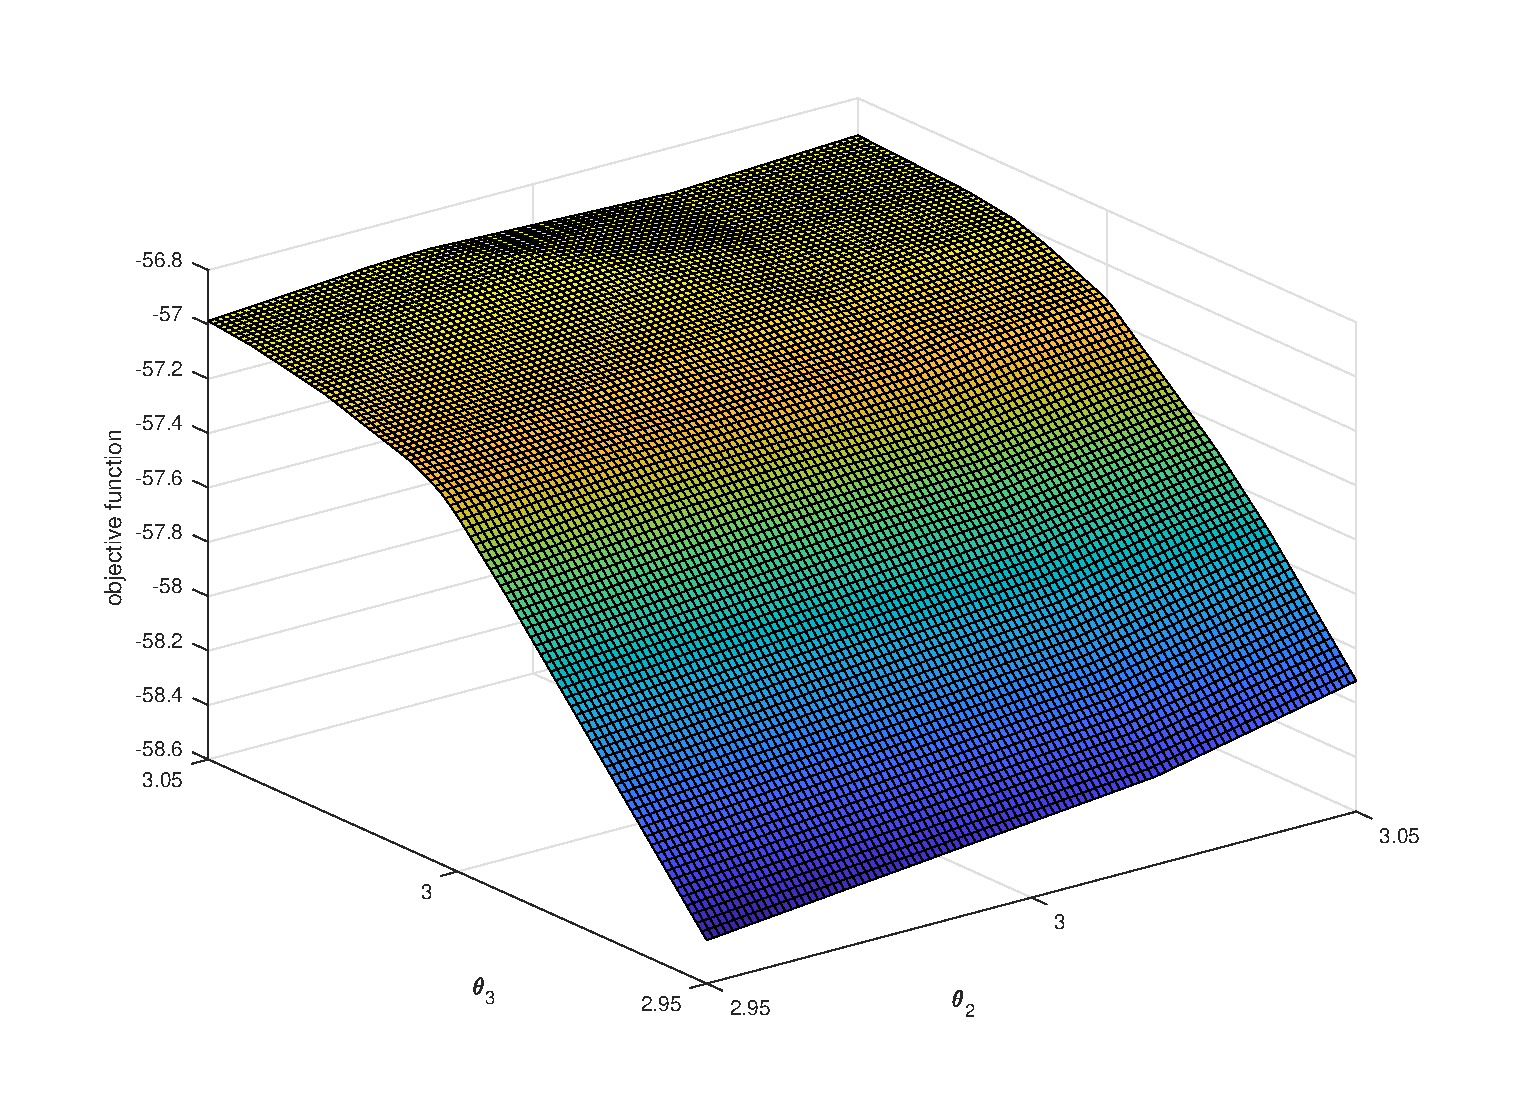
\includegraphics[width=0.9\textwidth]{figures/mesh.eps}
    \caption{Surface of objective function}
    \label{fig:lte-mean}
\end{figure}
\end{frame}

\section{Iterative Linear programming}
\begin{frame}{Iterative linear programming}
   Buchinsky (1994) proposed ILP to solve censored quantile regression.
    \begin{enumerate}
    \item Start with some $\hat{\theta}^{(0)}$ for $j=0$.
    \item Compute $X\hat{\theta}^{(j)}$ and collect the subsample $S_j = \{ i: x_i^{'}\hat{\theta}^{(j)}\geq 0 \}$.
    \item Use only subsample $S_j$, run the standard quantile regression with linear programming. With new $\hat{\theta}^{(j+1)}$, compute $S_{j+1}$.
    \item If $S_{j+1} = S_j$, then stop and set estimate to $\hat{\theta}^{(j+1)}$. Otherwise, set $j=j+1$ and repeat step.3.
\end{enumerate}
\end{frame}

\section{Quasi-Bayesian method}
\begin{frame}{Quasi-Bayesian method}
    Choose prior uniform over $\Theta = [\theta_0-10,\theta_0+10]$, use
    \begin{equation*}
        p_n(Y_i,X_i,\theta)=\frac{e^{nQ_n(Y_i,X_i,\theta)}\pi(Y_i,X_i,\theta)}{\int_{\Theta}e^{nQ_n(Y_i,X_i,\theta)}\pi(Y_i,X_i,\theta)\mbox{ d}\theta }
    \end{equation*}
    as posterior, run MCMC.

    Each parameter is updated via Gibss-Metroplis procedure, which modifies slightly the basic Metroplis-Hastings algorithm: for each update, only update one component each time. Adjust variance of innovation every 200 draws so that the rejection probability is roughly 50\%.
    
\end{frame}

\section{Results}
\begin{frame}{Performance of QBE and ILP}
    \begin{table}
        \centering
        \begin{tabular}{llll}
          \hline
                     & RMSE   & MAD    & mean bias \\ \hline
          n = 400    &        &        &  \\
          QBE-mean   & 1.9882 & 0.5445 & 0.5651    \\
          QBE-median & 1.6338 & 0.4796 & 0.4120    \\
          ILP (18)   & 0.9424 & 0.2867 & 0.0345    \\
                     & 3.1080 & 0.9505 & 0.0845    \\ \hline
          n = 1600   &        &        &  \\
          QBE-mean   & 0.3067 & 0.1051 & 0.0933    \\
          QBE-median & 0.2913 & 0.1004 & 0.0717    \\
          ILP (11)   & 0.2236 & 0.0742 & 0.0071    \\
                     & 2.6528 & 0.7371 & 0.0234    \\ \hline
        \end{tabular}
        \caption{ex}
    \end{table}
\end{frame}


\end{document}

